\section{General Modeling Overview}\label{general-modeling-overview}

The EnergyPlus program is a collection of many program modules that work together to calculate the energy required for heating and cooling a building using a variety of systems and energy sources. It does this by simulating the building and associated energy systems when they are exposed to different environmental and operating conditions. The core of the simulation is a model of the building that is based on fundamental heat balance principles. Since it is relatively meaningless to state: ``based on fundamental heat balance principles'', the model will be described in greater detail in later sections of this document in concert with the C++ code which is used to describe the model. It turns out that the model itself is relatively simple compared with the data organization and control that is needed to simulate the great many combinations of system types, primary energy plant arrangements, schedules, and environments. The next section shows this overall organization in schematic form. Later sections will expand on the details within the blocks of the schematic.

\begin{figure}[hbtp] % fig 1
\centering
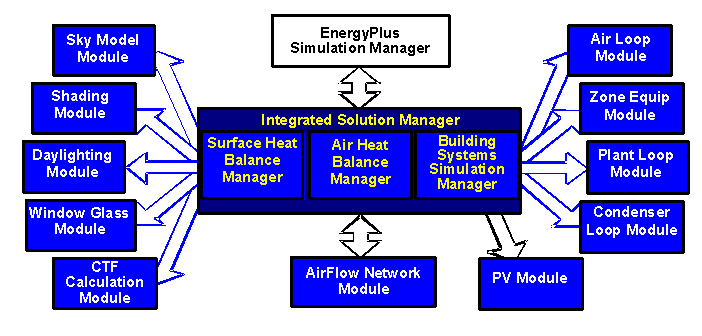
\includegraphics[width=0.9\textwidth, height=0.9\textheight, keepaspectratio=true]{media/image1.png}
\caption{EnergyPlus Program Schematic \protect \label{fig:energyplus-program-schematic}}
\end{figure}

